\chapter{Rephotography Application}

This chapter will document the development of the iOS application implementing
the theory outlined in the previous chapter. The iOS platform will be briefly
introduced before the user interface, features and implementation of the app
will be described.

\section{iOS Overview}
\newcommand*{\code}[1]{\texttt{#1}}

iOS is the operating system running on all of Apple's mobile devices. It is
currently\footnote{\today\ \citep{ios8}} at version 8.4.1 with its successor iOS
9 in beta stadium. Code is compiled by the clang compiler families and thus all
languages supported by this compiler can be used. The primary development
language is Objective-C, a strict, object-oriented superset of the C language\footnote{There is
   no precise definition which C version it is a superset of, except that it is
   ANSI standardised; For each C version supported by the compiler, Objective-C
will be compatible with it.}. Code of these languages can be freely mixed. An
Objective-C++ dialect exists to support C++ as well.

The software development kit for the platform employs Objective-C for most
high-level APIs and C for more low-level functionality. In regards to
application design, the Model-View-Controller (see \autoref{fig:mvc}) pattern is
used throughout the Cocoa library which incorporates the standard
(\code{Foundation} classes) and graphical user interface (\code{AppKit} on OSX,
\code{UIKit} on iOS) libraries as well as \code{Core Data} for persistence. For
applications with little or no need for data manipulation, the controller
objects can also fill the role of the model.  For every view hierarchy, a view
controller must exist to present it to the user and mediate interaction with
them.

\begin{figure}[h]
   {\centering      
      \newlength{\nodedist}
\setlength{\nodedist}{5cm}
\newlength{\defaultpgflinewidth}
\setlength{\defaultpgflinewidth}{\pgflinewidth}
\begin{tikzpicture}[
      mynode/.style={
         text width=3cm,
         text centered,
         draw,
         rounded corners=5pt,
         shape=rectangle,
         minimum width=1cm,
         text depth=2cm,
         inner sep=5pt,
         outer sep=3,
      },
      node distance=\nodedist,
      arrow label/.style={
         midway,
         fill=white,
         draw,
         shape=rectangle,
         rounded corners=3pt,
         line width=\defaultpgflinewidth,
         draw=black,
         text=black,
      },
      arrow/.style={
         line width=1.7pt,
         ->,
         RoyalBlue
      },
   ]
   \draw (0,0) node[mynode] (model) {
      \makebox[3cm]{Model}\\
      \hrulefill \\
      \texttt{Core} \texttt{Data}
   };
   \node[mynode,right=of model] (view) {
      \makebox[3cm]{View}\\
      \hrulefill \\
      \texttt{UIKit} : \texttt{UIView}
   };

   \node[mynode] (controller) at ($(model) !0.5! (view) + (0,-\nodedist)$) {
      \makebox[3cm]{Controller}\\
      \hrulefill \\
      \texttt{UIKit} : \texttt{UIViewController}
   };
   \draw [ arrow ] (controller.west) to [ bend left  ] node [ arrow label ] {Change state} (model.south);
   \draw [ arrow ] (controller.east) to [ bend right ] node [ arrow label ] {Update display} (view.south);
   \draw [ arrow ] (view.west) to       [ bend right ] node [ arrow label ] {Send user input} (controller.north);
   \draw [ arrow ] (view.north) to      [ bend right ] node [ arrow label ] {Request state} (model.north);
   \draw [ arrow ] (model.east) to      [ bend left  ] node [ arrow label ] {Notify of change} (view.north west);

\end{tikzpicture}


      \caption{Model-View-Controller pattern}
   \label{fig:mvc}}
\end{figure}

Generally, an iOS application is a sequence of view controllers presented to the
user in various ways---some may be full-fledged screens, while others are only
presented modally. Apple's XCode integrated development environment allows to
visually model the flow of the application by use of \code{Storyboard}s. These
are XML files which define controllers and their relationships. While
it is equally possible to specifiy the presentation order programmatically, this
allows for a cleaner separation between user interface and business logic.
Storyboards consist of a number of view controllers with associated views which
are connected by \code{Segue}s. A Segue is triggered by actions like a button
press and will present the next view controller to the user. The Storyboard for
the application developed in this work is shown in \autoref{fig:storyboard}.

\begin{figure}[h]
   {\centering      
      \begin{tikzpicture}[
      spy using outlines={circle,
         RoyalBlue,
         magnification=2,
         size=8cm,
      }
   ]
   \node[anchor=north west,inner sep=0] at (0,0) {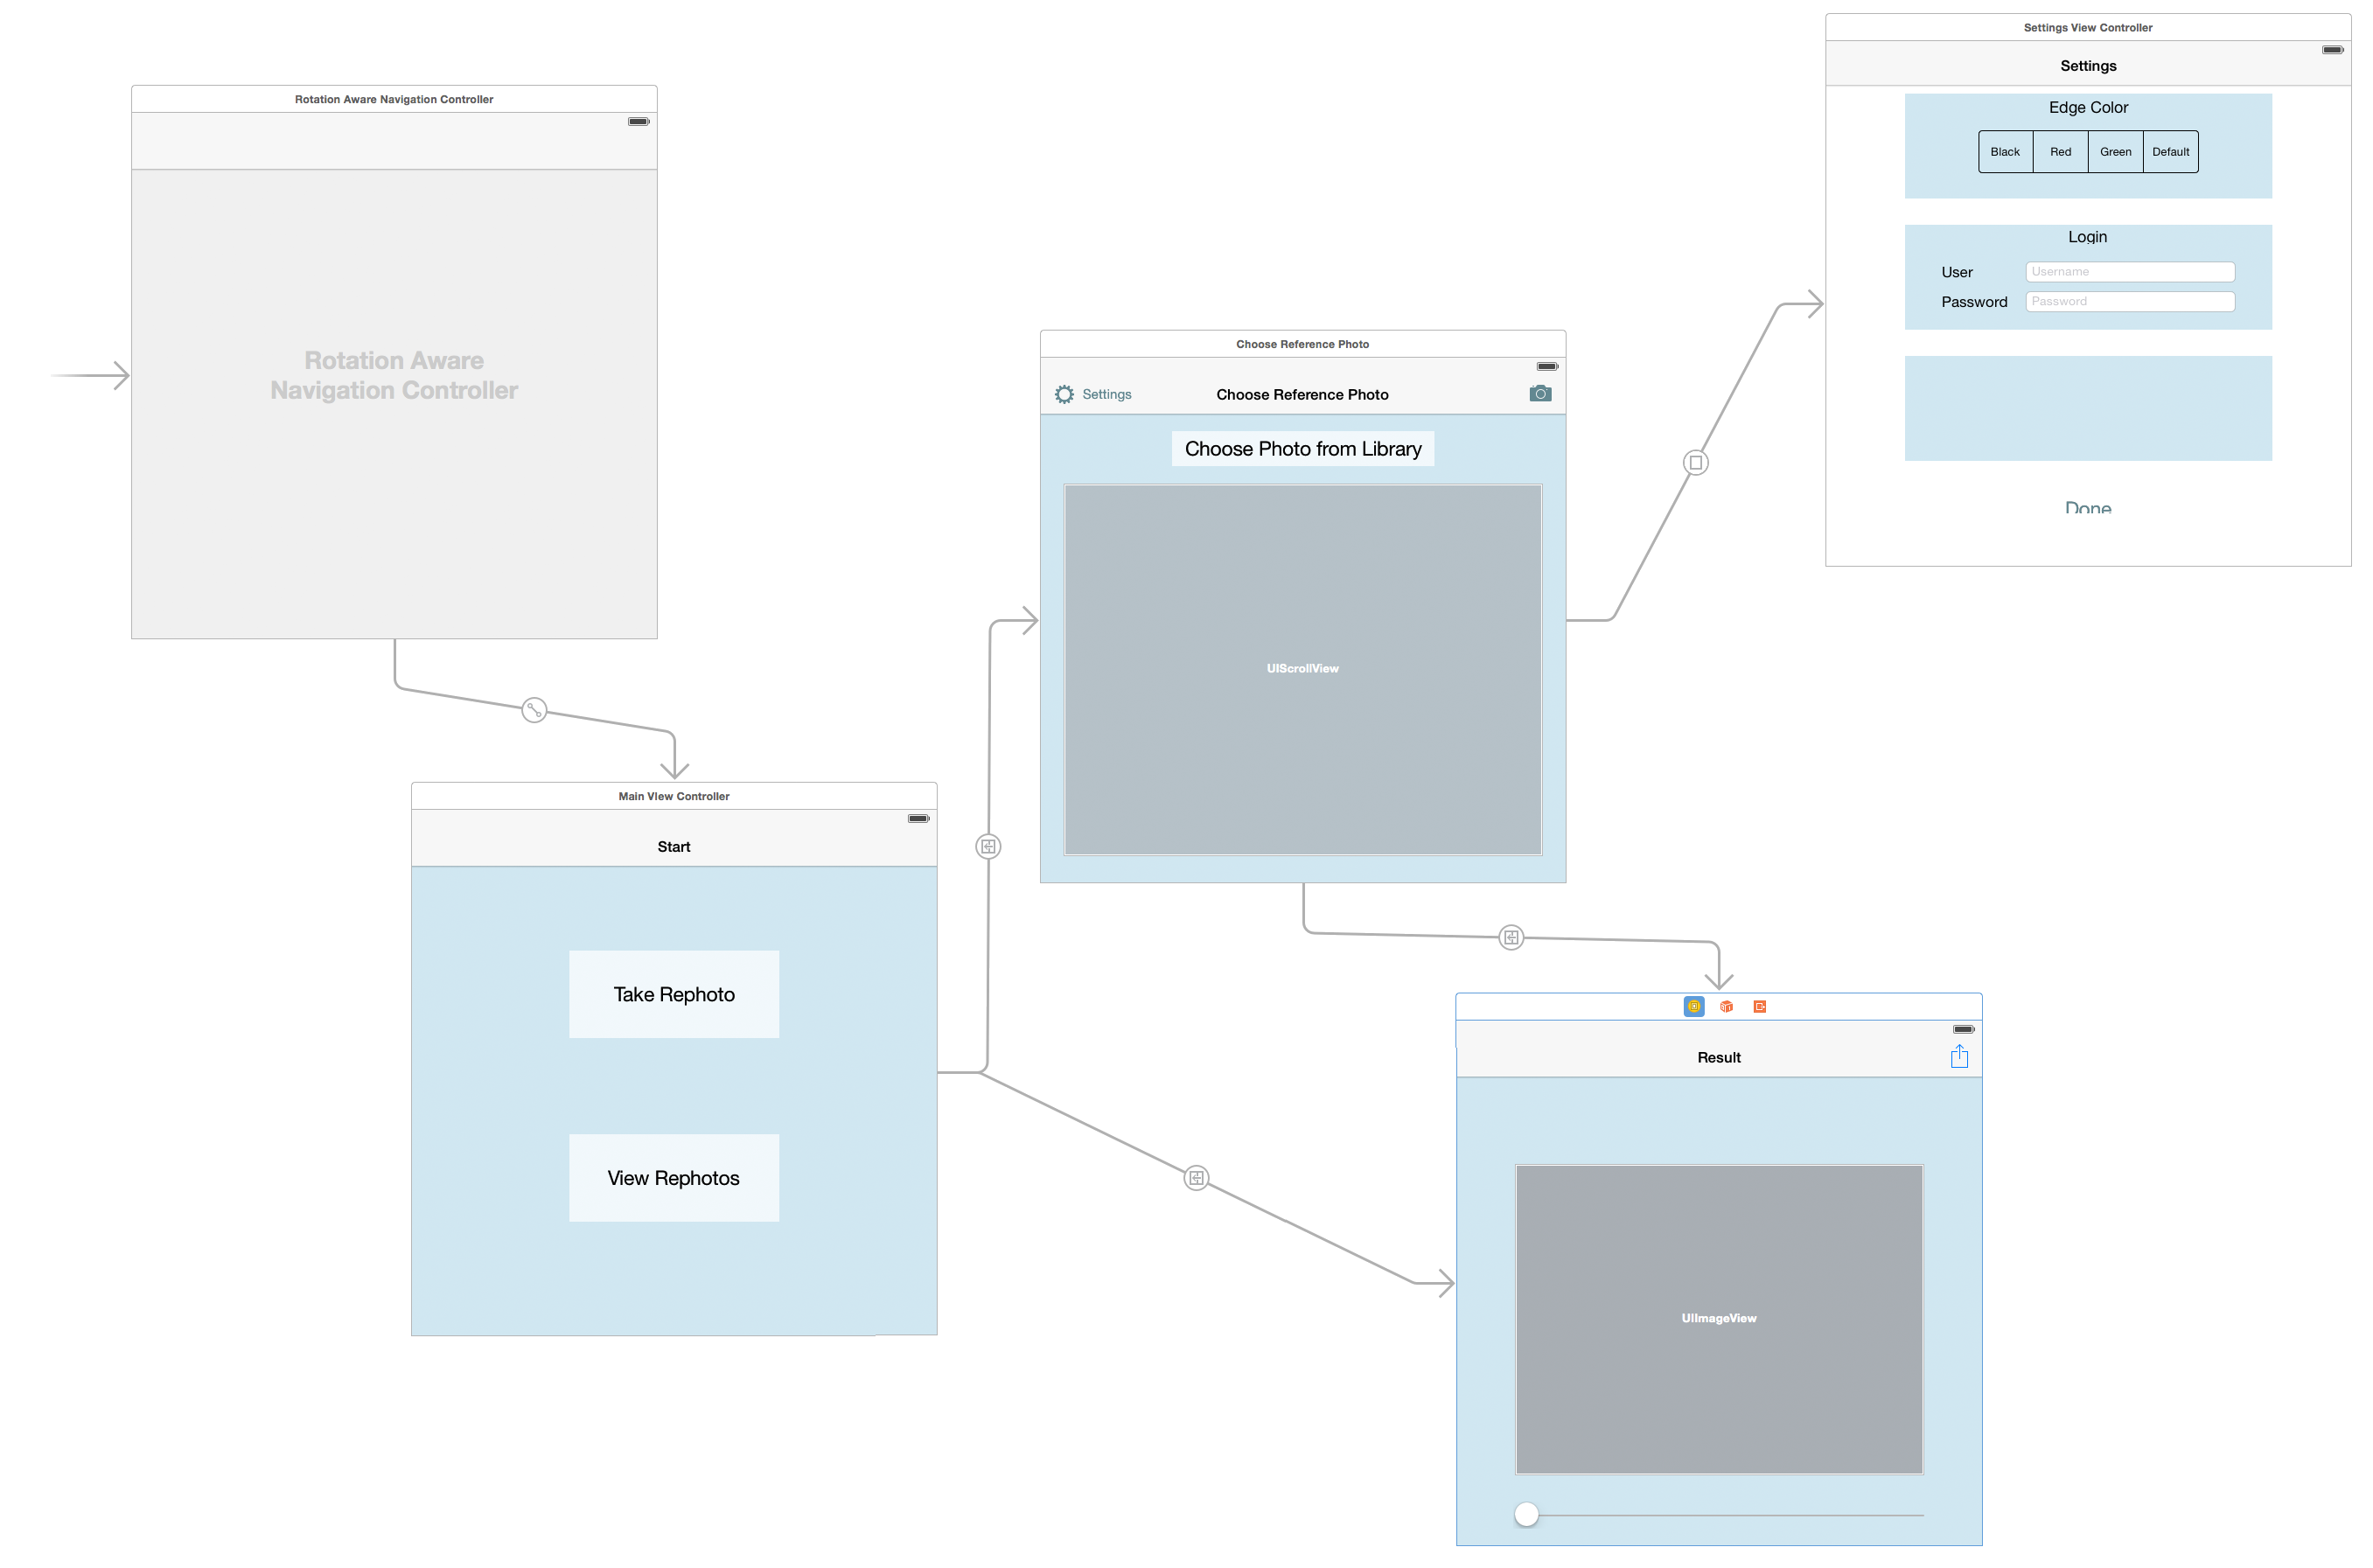
\includegraphics[width=\textwidth]{gfx/storyboard.png}};
   \spy[
      every spy on node/.append style={ultra thick},
      spy connection path={
         \draw[ultra thick] (tikzspyonnode) -- (tikzspyinnode);
      }
   ] on (6.5,-3) in
   node[fill=white,ultra thick] at (6,-10);
\end{tikzpicture}

      \caption[Storyboard example]{The Storyboard of this application. There is
      always a root view controller on whose stack new controllers are pushed or popped from.}
   \label{fig:storyboard}}
\end{figure}

\section{Software Modules}

Although Objective-C does not support modularisation by packages, namespace or
similar, the software can be divided into five parts.

\subsection{User Interface}

For the user interface, several custom views classes are implemented.
\begin{enumerate}
   \item \code{ArrowView} A view which is backed by an \code{ArrowLayer} and
      allows to display it as \code{CALayer}s cannot be shown without a
      wrapping \code{UIView}.
   \item \code{ArrowLayer} A \code{CALayer} subclass which can display a
      parametrisable arrow shape whose parameters can be seamlessly animated.
      \code{CALayers} are the backbone of all \code{UIView} objects.
   \item \code{ImageScrollView} A \code{ScrollView} subclass which allows to
      display a zoomable and pannable image while also preserving the visible
      portion when the user interface orientation changes.
   \item \code{CircleView} A simple view purely for drawing a circle parametrised
      with colour and line width.
   \item \code{MaskableUIImageView} An \code{UIImageView} which allows the
      image to be clipped to some percentage of its width. This is used to
      display a before-after comparison of the original and repeat photographs.
\end{enumerate}

Furthermore, two view hierarchies and the Storyboard belong to this module.  If
a custom view must exhibit some particular behviour which necessitates custom
methods, creating classes is appropriate. For interface elements which contain a
larger hierarchy of nested views without exposing any particular behaviour,
specifying them in a visual fashion is less involved. Such view hierarchies can
be built visually as \code{XIB} files in an XML format. The
\code{CameraOverlay} overlayed on the current camera picture is created like
this, as well as the launch screen shown when starting the app.

\subsection{Image Processing}

For all image processing, the OpenCV library used in version 3.0. The library
can be natively used from C++, but Python and Java bindings as well as a
deprecated C API exist. OpenCV encodes images in its \code{Mat} type which is
the only type perforating other parts of the application. 
While it is possible to mix Objective-C and C++ code,
using C++ types in header files forces every client including them to also be
compiled as Objective-C++ which may be unwanted. For instance, XCode's
refactoring tools cannot be used on these sources. It is thus reasonable to create
wrapper classes for all C++ types encapsulating the access to the data so that
the interface is pure Objective-C. Only the implementation of the wrapper class
would need to be compiled as C++, no client would be affected. Ideally, all
access to C++ types could be mediated this way, but often this would necessitate 
a large amount of boilerplate code to translate Objective-C messages in C++
calls to the wrapped object.
It is therefore convenient to encapsulate a C++ type but make it still accessible to
client classes if needed. 

One solution is a variant of the \emph{Pointer-to-Implementation} pattern
(PIMPL, also known as \emph{Bridge} in \citep{gamma1995}). The wrapper class'
interface (\autoref{lst:pimpl}) is specified in pure Objective-C and contains a
opaque pointer to a C \code{struct} representing the wrapped data as a C type
which therefore does not lead to compatibility issues as all C code is valid
Objective-C. The definition of this pointer-to-implementation type is placed in
a second header file (\autoref{lst:pimpl2}) and is imported only by those
clients which actually need to access the data, not only pass it on. This
permits to compile only those source files as Objective-C++ which must deal with
the actual OpenCV \code{Mat}. In principle, it would be possible to create
methods in the wrapper class for all uses of the C++ type throughout the
program. However, this would waste the benefits which e.g. C++ operator
overloading yields for readability. Since all image processing is done in C++
anyway, it is more economic to simply provide access to the wrapped data to
those classes that need it.

\lstset{
   language=[Objective]C,
   float,
}

\begin{lstlisting}[
   caption={\code{CVMatWrapper.h}. The wrapper interface contains an opaque pointer to a C
      \code{struct}. \code{\#include}ing this header does not invalidate
   othewise valid Objective-C code.},
   label={lst:pimpl},
]
struct CVMatWrapperImpl;
@interface CVMatWrapper : NSObject
@property (nonatomic,readwrite) struct CVMatWrapperImpl* impl; ///< Pointer to struct wrapping the matrix
@property (nonatomic,readonly) int rows; ///< Number of rows of the wrapped matrix
@property (nonatomic,readonly) int cols; ///< Number of columns of the wrapped matrix
-(NSArray*)eulerAngles;
-(NSString*)description;
@end
\end{lstlisting}

\begin{lstlisting}[
   caption={\code{CVMatWrapperImpl.h}. The implementation header defines the actually wrapped type.
      Including it will force a client to compile as Objective-C++ since a C++
      type is used. Every class which deals with the data itself can include this
   header in addition to the wrapper one.},
   label={lst:pimpl2},
]
struct CVMatWrapperImpl
{
   cv::Mat cvMatrix; ///< The wrapped matrix
};
\end{lstlisting}

\begin{lstlisting}[
   caption={\code{CVMatWrapper.mm}. The wrapper class' implementation must be Objective-C++ and can
   encapsulate all access to the underlying data, if necessary.},
   label={lst:pimpl3},
]
#import "CVMatWrapper.h"
#import "CVMatWrapperImpl.h"

@implementation CVMatWrapper
-(instancetype)init
{
   self = [super init];
   if (self) self.impl = new CVMatWrapperImpl; // allocate the struct wrapping the matrix
   return self;
}

-(void)dealloc
{
   if (self.impl)
   delete self.impl;
}

-(NSString*)description
{
   //...
}

-(NSArray*)eulerAngles
{
   // ...
}

-(int)rows
{
   return (self.impl->cvMatrix).rows;
}

-(int)cols
{
   return (self.impl->cvMatrix).cols;
}
@end
\end{lstlisting}

The bulk of the work is done inside the utility class' \code{ImageUtils} static
methods. To compute the pose difference between two frames, clients can call the
public method
\code{+[computePoseDifferenceBetweenCamera:
secondCamera:calibrationFile:scale:]}. The two images must be passed, as well as
the path to a calibration file in OpenCV's \code{FileStorage} format. A scale
parameter can be used to speed up the computation by downsampling the images.
Internally, the method converts the images, uses OpenCV image processing
functions to compute the pose difference and the average distance of the matched
features to the first camera. The client is returned an \code{NSDictionary}
containing the rotation, translation, average point distance, and---should the
computation fail---an error code in which case all other values are invalid.

\subsection{View Controllers}

\subsection*{\code{MainViewController}}

\newcommand*{\button}[1]{
   \tikzexternaldisable
   \tikz[baseline=-.5ex]{\node[inner sep=1pt,outer sep=0,draw,rounded corners=2pt]{\small\texttt{#1}};}
   \tikzexternalenable
}

When the app starts up, the user is shown a \code{MainViewController} which
offers a choice whether to make a new rephotograph or view existing ones.
Clicking the \button{Take Rephoto} button will trigger a segue to a
\code{PhotoChooserController}, while tapping \button{View Rephotos} will modally
present an \code{ELCImagePickerController}.

\subsection*{\code{PhotoChooserController}}

This view controller displays a scrollable and pannable view and a
button \button{Choose Photo from Library} to
load a reference photograph into it. The photo is picked from the user's photo album.
Tapping 
Furthermore, the navigation bar contains a button to access the settings
(\raisebox{-3pt}{
\includegraphics[width=1em]{gfx/settings_icon.png}}, see below) as well as a
button to start the rephotograph
(\raisebox{-1pt}{
\includegraphics[width=1em]{gfx/cam_icon.png}}).

When an image is picked, the controller uses the Canny edge detection algorithm
\citep{canny1986} to generate an overlay which will then help the user in
finding the perfect aligment.

\subsection*{\code{SettingsViewController}}

The \code{SettingsViewController} possesses three panels which allow to
modify the color of the edge overlay and insert authentication data for
future use with an envisioned online platform. The third panel is unused in the current
version and can be used for other kinds of preferences such as the default type
of visualisation for the necessary camera motion.

\subsection*{\code{ResultViewController}}

This controller must be passed a completed rephotograph in an \code{ImageData}
object and displays the new image over the orginal. With a slider, the new image
is horizontally clipped to some percentage of it width and can thus be
dynamically unrolled over the original.

\subsection*{\code{ELCImagePickerController}}

For the task of reviewing rephotographs, the \code{ELCImagePickerController} is
used. Contrarily to the built-in \code{UIImagePickerController}, this
reimplementation by \citet{nutting2013} allows to display a specific asset, like
a photo album instead of all assets there are. In the album display, the user is
shown the new photographs of each rephoto and upon selection is presented a
\code{ResultViewController}

\subsection{Categories}

Code reuse in Objective-C can be accomplished by inheritance as in other
object-oriented languages, but often, when only one piece of behaviour is to be
added, not overridden\footnote{The behaviour is undefined when a Category method
has the same signature as one of the class \citep{customizing}}, the
lightweight Category concept is employed. A Category on a class adds methods
or properties to that class The header file declaring the category can be
included by all clients that wish to make use of the modified or added
behaviour, and left out by all others. This way, no unnecessarily large class
hierarchy is created.

In this application, categories are used for different purposes. They are
summarised in \autoref{tab:categories}.

      \rowcolors{2}{gray!5}{white} % alternating colours
\begin{table}
   \begin{tabularx}{\linewidth}{>{\ttfamily}p{4cm}X}
      \toprule
      \rowcolor{white}
      {\rmfamily Category Name}           & Function \\
      \midrule
      NSMutableURLRequest (RephotoUpload) & Adds method to post an rephoto to an
      experimental server via HTTP \\
      ALAssetsLibrary (CustomPhotoAlbum)  & Adds method to add an image to a
      specific album, not possible per default. Used to save rephotos to the
      \code{Rephotos} album \\
      NSUserDefaults (UIColor)            & By default, only some types can be
      persistently saved in the user defaults. Adds method to save colours. \\
      CALayer (UIColor)                   & Properties for view objects can be
      set in Interface Builder, but only if they are of object type. To set a
      view's backing layer's border colour outside of the code, a colour
      property of object type is defined, mapped to the C type \code{CGColor}
      used by \code{CALayer}. \\
      UIBezierPath (Arrow)                & Adds a method to generate an arrow
      shape with a bézier curve. \\
      UIImage (Zoom)                      & Adds a method to crop an image to a
      rectangle centered on the image center, effectively zooming in. \\
      UIScrollView (Center)               & Adds methods to center the content
      and zoom to a particular size \\
      UIColor (CustomColors)              & Contrary to Android, iOS possesses
      no Resources framework, so this Category declares some commonly used
      colours for the user interface \\
      UIView (Effects)                    & Adds some animation methods to all
      views to avoid repeating boilerplate code \\
      \bottomrule
   \end{tabularx}
   \caption{Summary of categories}
   \label{tab:categories}
\end{table}

\subsection{Other Classes}


